\upaper{49}{The Inhabited Worlds}
\uminitoc{The Planetary Life}
\uminitoc{Planetary Physical Types}
\uminitoc{Worlds of the Nonbreathers}
\uminitoc{Evolutionary Will Creatures}
\uminitoc{The Planetary Series of Mortals}
\uminitoc{Terrestrial Escape}
\author{Melchizedek}
\vs p049 0:1 All mortal\hyp{}inhabited worlds are evolutionary in origin and nature. These spheres are the spawning ground, the evolutionary cradle, of the mortal races of time and space. Each unit of the ascendant life is a veritable training school for the stage of existence just ahead, and this is true of every stage of man’s progressive Paradise ascent; just as true of the initial mortal experience on an evolutionary planet as of the final universe headquarters school of the Melchizedeks, a school which is not attended by ascending mortals until just before their translation to the regime of the superuniverse and the attainment of first\hyp{}stage spirit existence.
\vs p049 0:2 \pc All inhabited worlds are basically grouped for celestial administration into the local systems, and each of these local systems is limited to about 1,000 evolutionary worlds. This limitation is by the decree of the Ancients of Days, and it pertains to actual evolutionary planets whereon mortals of survival status are living. Neither worlds finally settled in light and life nor planets in the prehuman stage of life development are reckoned in this group.
\vs p049 0:3 \pc Satania itself is an unfinished system containing only 619 inhabited worlds. Such planets are numbered serially in accordance with their registration as inhabited worlds, as worlds inhabited by will creatures. Thus was Urantia given the number \bibemph{606 of Satania,} meaning the 606\ts{th} world in this local system on which the long evolutionary life process culminated in the appearance of human beings. There are 36 uninhabited planets nearing the life\hyp{}endowment stage, and several are now being made ready for the Life Carriers. There are nearly 200 spheres which are evolving so as to be ready for life implantation within the next few million years.
\vs p049 0:4 Not all planets are suited to harbour mortal life. Small ones having a high rate of axial revolution are wholly unsuited for life habitats. In several of the physical systems of Satania the planets revolving around the central sun are too large for habitation, their great mass occasioning oppressive gravity. Many of these enormous spheres have satellites, sometimes a half dozen or more, and these moons are often in size very near that of Urantia, so that they are almost ideal for habitation.
\vs p049 0:5 The oldest inhabited world of Satania, world number 1, is Anova, one of the 44 satellites revolving around an enormous dark planet but exposed to the differential light of three neighbouring suns. Anova is in an advanced stage of progressive civilization.
\usection{The Planetary Life}
\vs p049 1:1 The universes of time and space are gradual in development; the progression of life --- terrestrial or celestial --- is neither arbitrary nor magical. Cosmic evolution may not always be understandable (predictable), but it is strictly nonaccidental.
\vs p049 1:2 The biologic unit of material life is the protoplasmic cell, the communal association of chemical, electrical, and other basic energies. The chemical formulas differ in each system, and the technique of living cell reproduction is slightly different in each local universe, but the Life Carriers are always the living catalysers who initiate the primordial reactions of material life; they are the instigators of the energy circuits of living matter.
\vs p049 1:3 All the worlds of a local system disclose unmistakable physical kinship; nevertheless, each planet has its own scale of life, no two worlds being exactly alike in plant and animal endowment. These planetary variations in the system life types result from the decisions of the Life Carriers. But these beings are neither capricious nor whimsical; the universes are conducted in accordance with law and order. The laws of Nebadon are the divine mandates of Salvington, and the evolutionary order of life in Satania is in consonance with the evolutionary pattern of Nebadon.
\vs p049 1:4 Evolution is the rule of human development, but the process itself varies greatly on different worlds. Life is sometimes initiated in one centre, sometimes in three, as it was on Urantia. On the atmospheric worlds it usually has a marine origin, but not always; much depends on the physical status of a planet. The Life Carriers have great latitude in their function of life initiation.
\vs p049 1:5 In the development of planetary life the vegetable form always precedes the animal and is quite fully developed before the animal patterns differentiate. All animal types are developed from the basic patterns of the preceding vegetable kingdom of living things; they are not separately organized.
\vs p049 1:6 The early stages of life evolution are not altogether in conformity with your present\hyp{}day views. \bibemph{Mortal man is not an evolutionary accident.} There is a precise system, a universal law, which determines the unfolding of the planetary life plan on the spheres of space. Time and the production of large numbers of a species are not the controlling influences. Mice reproduce much more rapidly than elephants, yet elephants evolve more rapidly than mice.
\vs p049 1:7 The process of planetary evolution is orderly and controlled. The development of higher organisms from lower groupings of life is not accidental. Sometimes evolutionary progress is temporarily delayed by the destruction of certain favourable lines of life plasm carried in a selected species. It often requires ages upon ages to recoup the damage occasioned by the loss of a single superior strain of human heredity. These selected and superior strains of living protoplasm should be jealously and intelligently guarded when once they make their appearance. And on most of the inhabited worlds these superior potentials of life are valued much more highly than on Urantia.
\usection{Planetary Physical Types}
\vs p049 2:1 There is a standard and basic pattern of vegetable and animal life in each system. But the Life Carriers are oftentimes confronted with the necessity of modifying these basic patterns to conform to the varying physical conditions which confront them on numerous worlds of space. They foster a generalized system type of mortal creature, but there are 7 distinct physical types as well as thousands upon thousands of minor variants of these 7 outstanding differentiations:
\vs p049 2:2 \ublistelem{1.}\bibnobreakspace Atmospheric types.
\vs p049 2:3 \ublistelem{2.}\bibnobreakspace Elemental types.
\vs p049 2:4 \ublistelem{3.}\bibnobreakspace Gravity types.
\vs p049 2:5 \ublistelem{4.}\bibnobreakspace Temperature types.
\vs p049 2:6 \ublistelem{5.}\bibnobreakspace Electric types.
\vs p049 2:7 \ublistelem{6.}\bibnobreakspace Energizing types.
\vs p049 2:8 \ublistelem{7.}\bibnobreakspace Unnamed types.
\vs p049 2:9 \pc The Satania system contains all of these types and numerous intermediate groups, although some are very sparingly represented.
\vs p049 2:10 \ublistelem{1.}\bibnobreakspace \bibemph{The atmospheric types.} The physical differences of the worlds of mortal habitation are chiefly determined by the nature of the atmosphere; other influences which contribute to the planetary differentiation of life are relatively minor.
\vs p049 2:11 The present atmospheric status of Urantia is almost ideal for the support of the breathing type of man, but the human type can be so modified that it can live on both the superatmospheric and the subatmospheric planets. Such modifications also extend to the animal life, which differs greatly on the various inhabited spheres. There is a very great modification of animal orders on both the sub\hyp{} and the superatmospheric worlds.
\vs p049 2:12 Of the atmospheric types in Satania, about 2.5\% are subbreathers, about 5\% superbreathers, and over 91\% are mid\hyp{}breathers, altogether accounting for 98.5\% of the Satania worlds.\tunemarkup{pictures}{\begin{figure}[H]\centering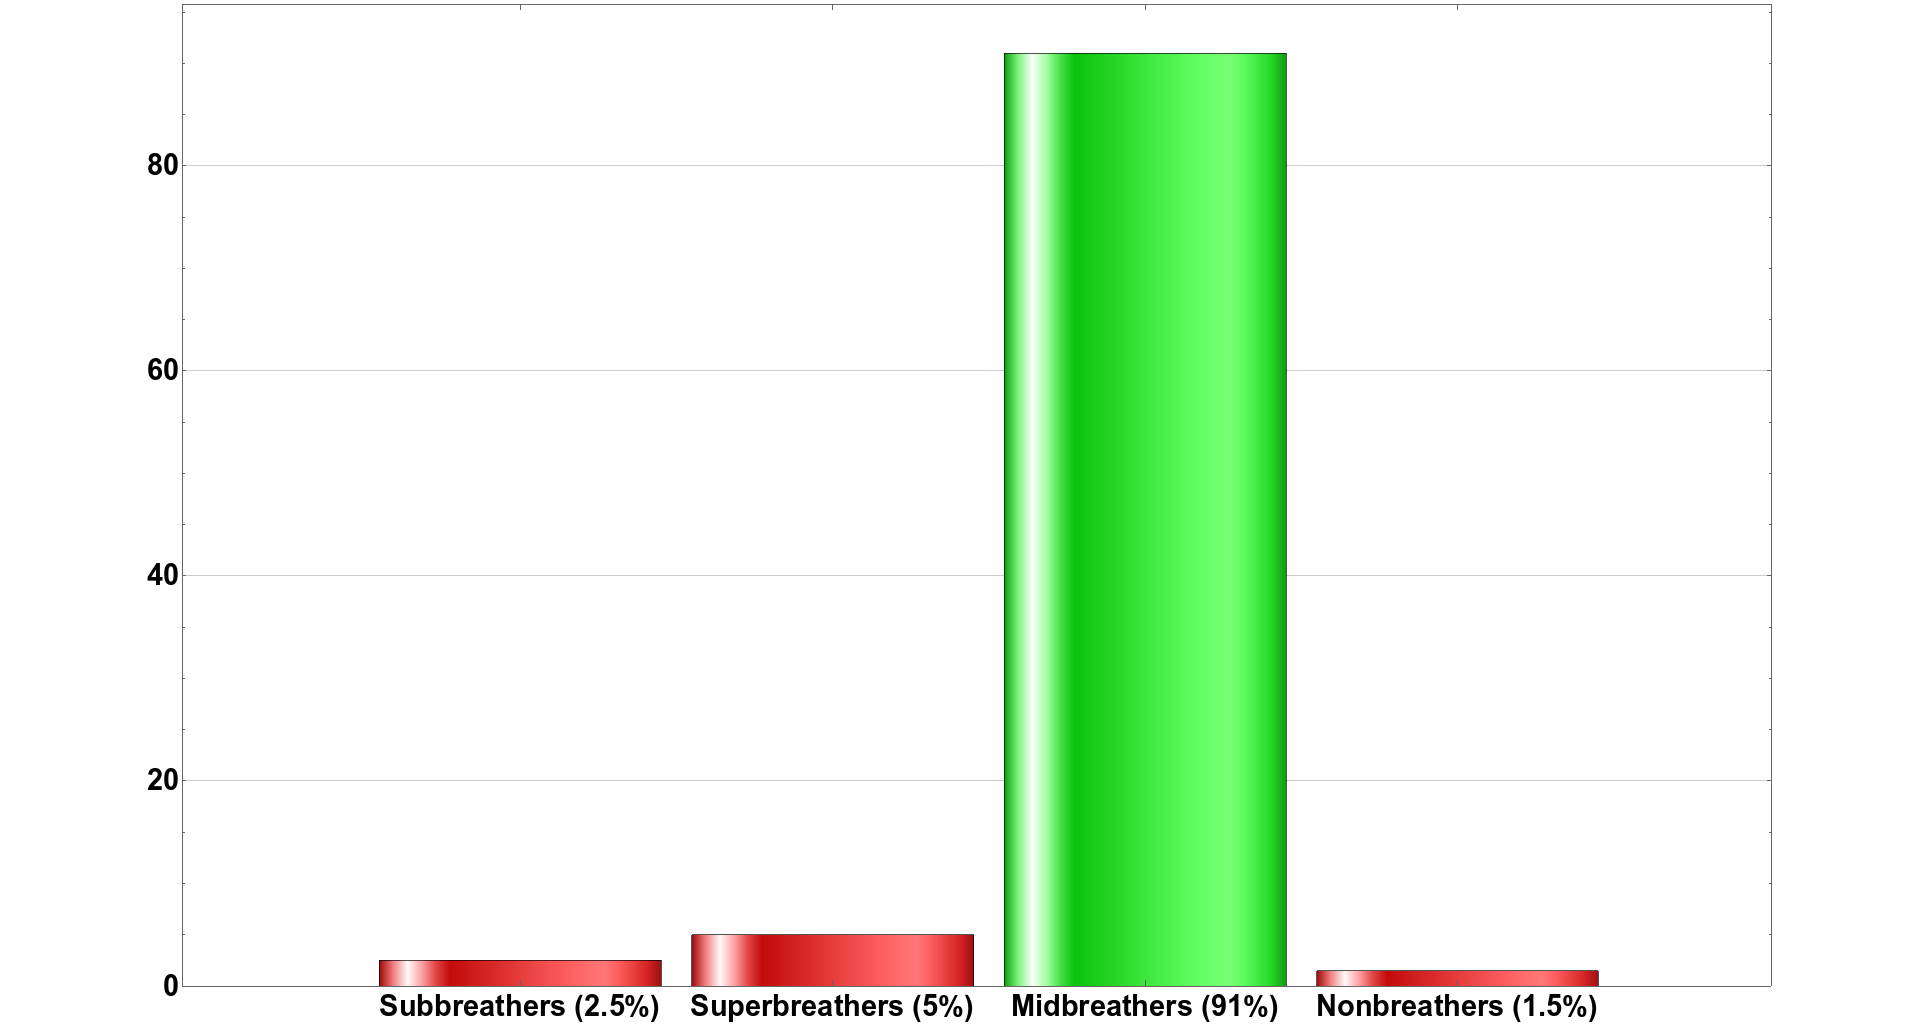
\includegraphics[width=\columnwidth]{images/breather-types.png}\caption{Distribution of Atmospheric Types (\%), Urantia type (``Midbreathers'') is marked with green.}\end{figure}}
\vs p049 2:13 Beings such as the Urantia races are classified as mid\hyp{}breathers; you represent the average or typical breathing order of mortal existence. If intelligent creatures should exist on a planet with an atmosphere similar to that of your near neighbour, Venus, they would belong to the superbreather group, while those inhabiting a planet with an atmosphere as thin as that of your outer neighbour, Mars, would be denominated subbreathers.
\vs p049 2:14 If mortals should inhabit a planet devoid of air, like your moon, they would belong to the separate order of nonbreathers. This type represents a radical or extreme adjustment to the planetary environment and is separately considered. Nonbreathers account for the remaining 1.5\% of Satania worlds.
\vs p049 2:15 \ublistelem{2.}\bibnobreakspace \bibemph{The elemental types.} These differentiations have to do with the relation of mortals to water, air, and land, and there are four distinct species of intelligent life as they are related to these habitats. The Urantia races are of the land order.
\vs p049 2:16 It is quite impossible for you to envisage the environment which prevails during the early ages of some worlds. These unusual conditions make it necessary for the evolving animal life to remain in its marine nursery habitat for longer periods than on those planets which very early provide a hospitable land\hyp{}and\hyp{}atmosphere environment. Conversely, on some worlds of the superbreathers, when the planet is not too large, it is sometimes expedient to provide for a mortal type which can readily negotiate atmospheric passage. These air navigators sometimes intervene between the water and land groups, and they always live in a measure upon the ground, eventually evolving into land dwellers. But on some worlds, for ages they continue to fly even after they have become land\hyp{}type beings.
\vs p049 2:17 It is both amazing and amusing to observe the early civilization of a primitive race of human beings taking shape, in one case, in the air and treetops and, in another, midst the shallow waters of sheltered tropic basins, as well as on the bottom, sides, and shores of these marine gardens of the dawn races of such extraordinary spheres. Even on Urantia there was a long age during which primitive man preserved himself and advanced his primitive civilization by living for the most part in the treetops as did his earlier arboreal ancestors. And on Urantia you still have a group of diminutive mammals (the bat family) that are air navigators, and your seals and whales, of marine habitat, are also of the mammalian order.
\vs p049 2:18 In Satania, of the elemental types, 7\% are water, 10\% air, 70\% land, and 13\% combined land\hyp{}and\hyp{}air types. But these modifications of early intelligent creatures are neither human fishes nor human birds. They are of the human and prehuman types, neither superfishes nor glorified birds but distinctly mortal.\tunemarkup{pictures}{\begin{figure}[H]\centering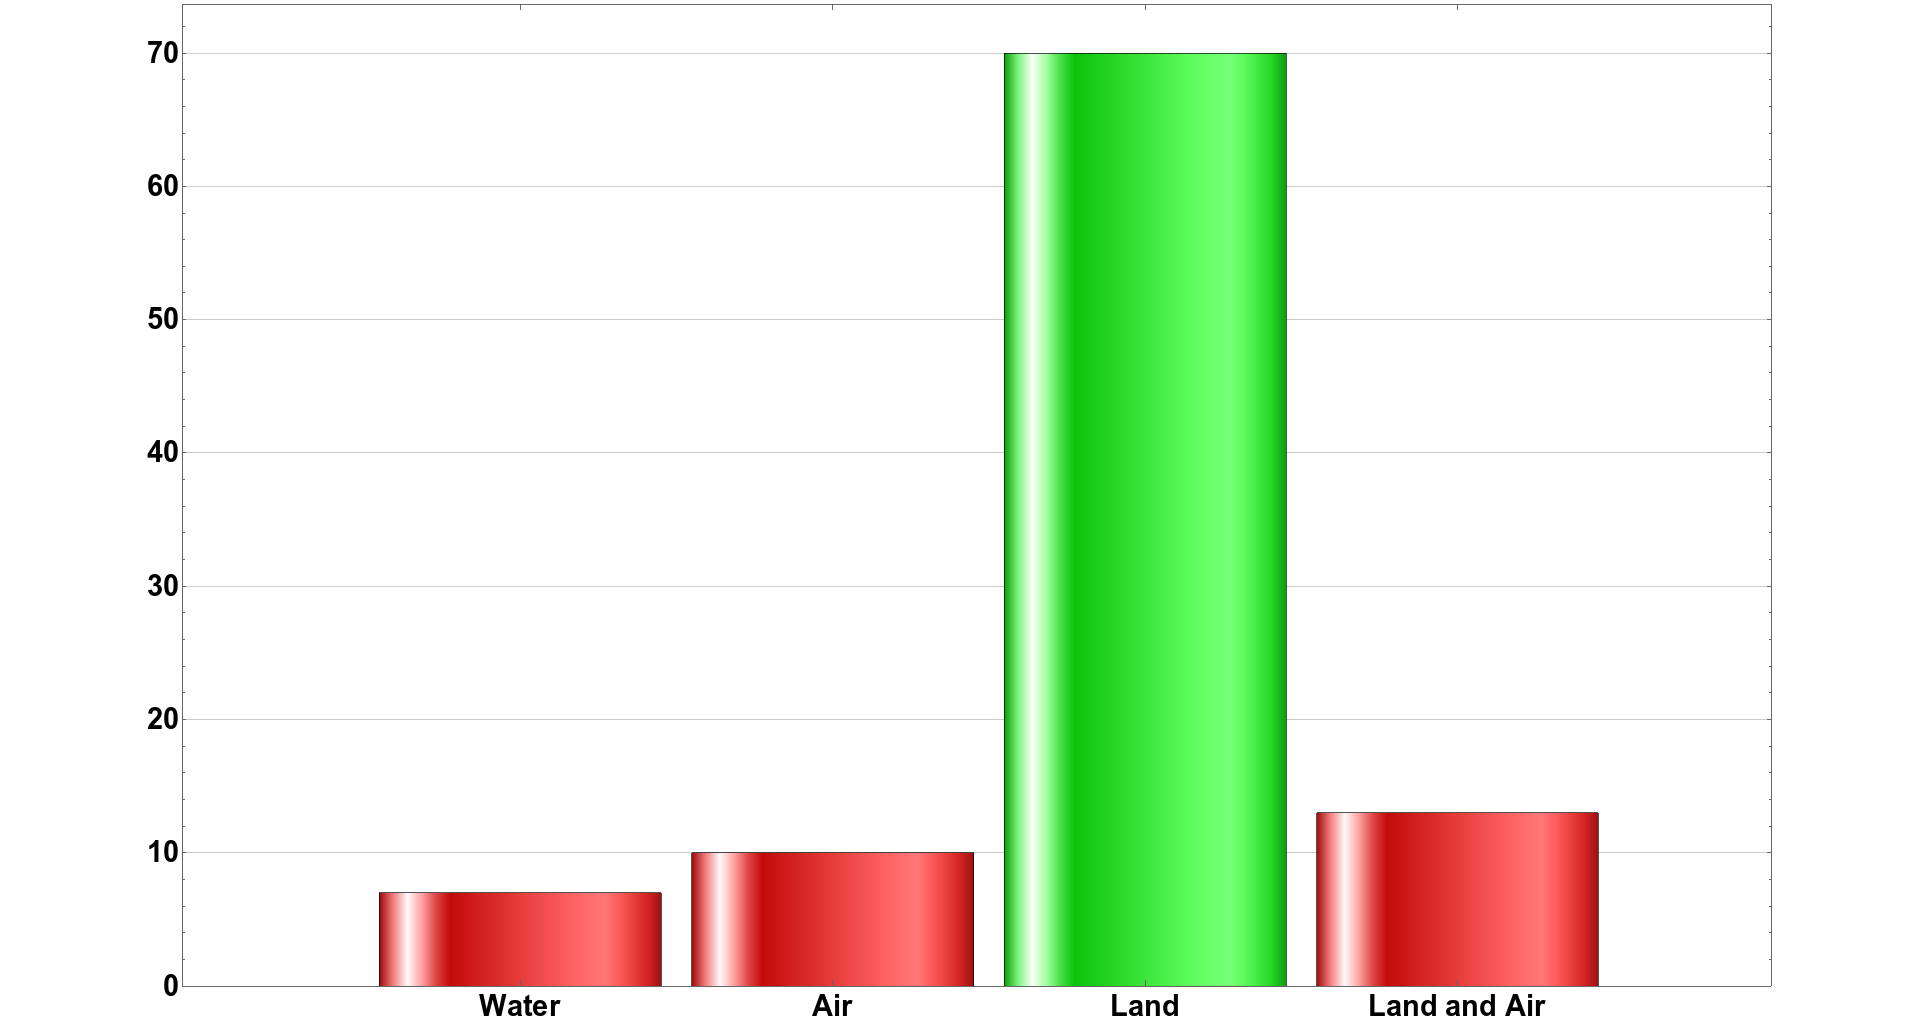
\includegraphics[width=\columnwidth]{images/elemental-types.png}\caption{Distribution of Elemental Types (\%), Urantia type (``Land'') is marked with green.}\end{figure}}
\vs p049 2:19 \ublistelem{3.}\bibnobreakspace \bibemph{The gravity types.} By modification of creative design, intelligent beings are so constructed that they can freely function on spheres both smaller and larger than Urantia, thus being, in measure, accommodated to the gravity of those planets which are not of ideal size and density.
\vs p049 2:20 The various planetary types of mortals vary in height, the average in Nebadon being a trifle under 2.1\,m. Some of the larger worlds are peopled with beings who are only about 76\,cm in height. Mortal stature ranges from here on up through the average heights on the average\hyp{}sized planets to around 3\,m on the smaller inhabited spheres. In Satania there is only one race under 1.2\,m in height. 20\% of the Satania inhabited worlds are peopled with mortals of the modified gravity types occupying the larger and the smaller planets.
\vs p049 2:21 \ublistelem{4.}\bibnobreakspace \bibemph{The temperature types.} It is possible to create living beings who can withstand temperatures both much higher and much lower than the life range of the Urantia races. There are five distinct orders of beings as they are classified with reference to heat\hyp{}regulating mechanisms. In this scale the Urantia races are number three. 30\% of Satania worlds are peopled with races of modified temperature types. 12\% belong to the higher temperature ranges, 18\% to the lower, as compared with Urantians, who function in the mid\hyp{}temperature group.
\vs p049 2:22 \ublistelem{5.}\bibnobreakspace \bibemph{The electric types.} The electric, magnetic, and electronic behaviour of the worlds varies greatly. There are ten designs of mortal life variously fashioned to withstand the differential energy of the spheres. These ten varieties also react in slightly different ways to the chemical rays of ordinary sunlight. But these slight physical variations in no way affect the intellectual or the spiritual life.
\vs p049 2:23 Of the electric groupings of mortal life, almost 23\% belong to class number 4, the Urantia type of existence. These types are distributed as follows: number 1, 1\%; number 2, 2\%; number 3, 5\%; number 4, 23\%; number 5, 27\%; number 6, 24\%; number 7, 8\%; number 8, 5\%; number 9, 3\%; number 10, 2\% --- in whole percentages.\tunemarkup{pictures}{\begin{figure}[H]\centering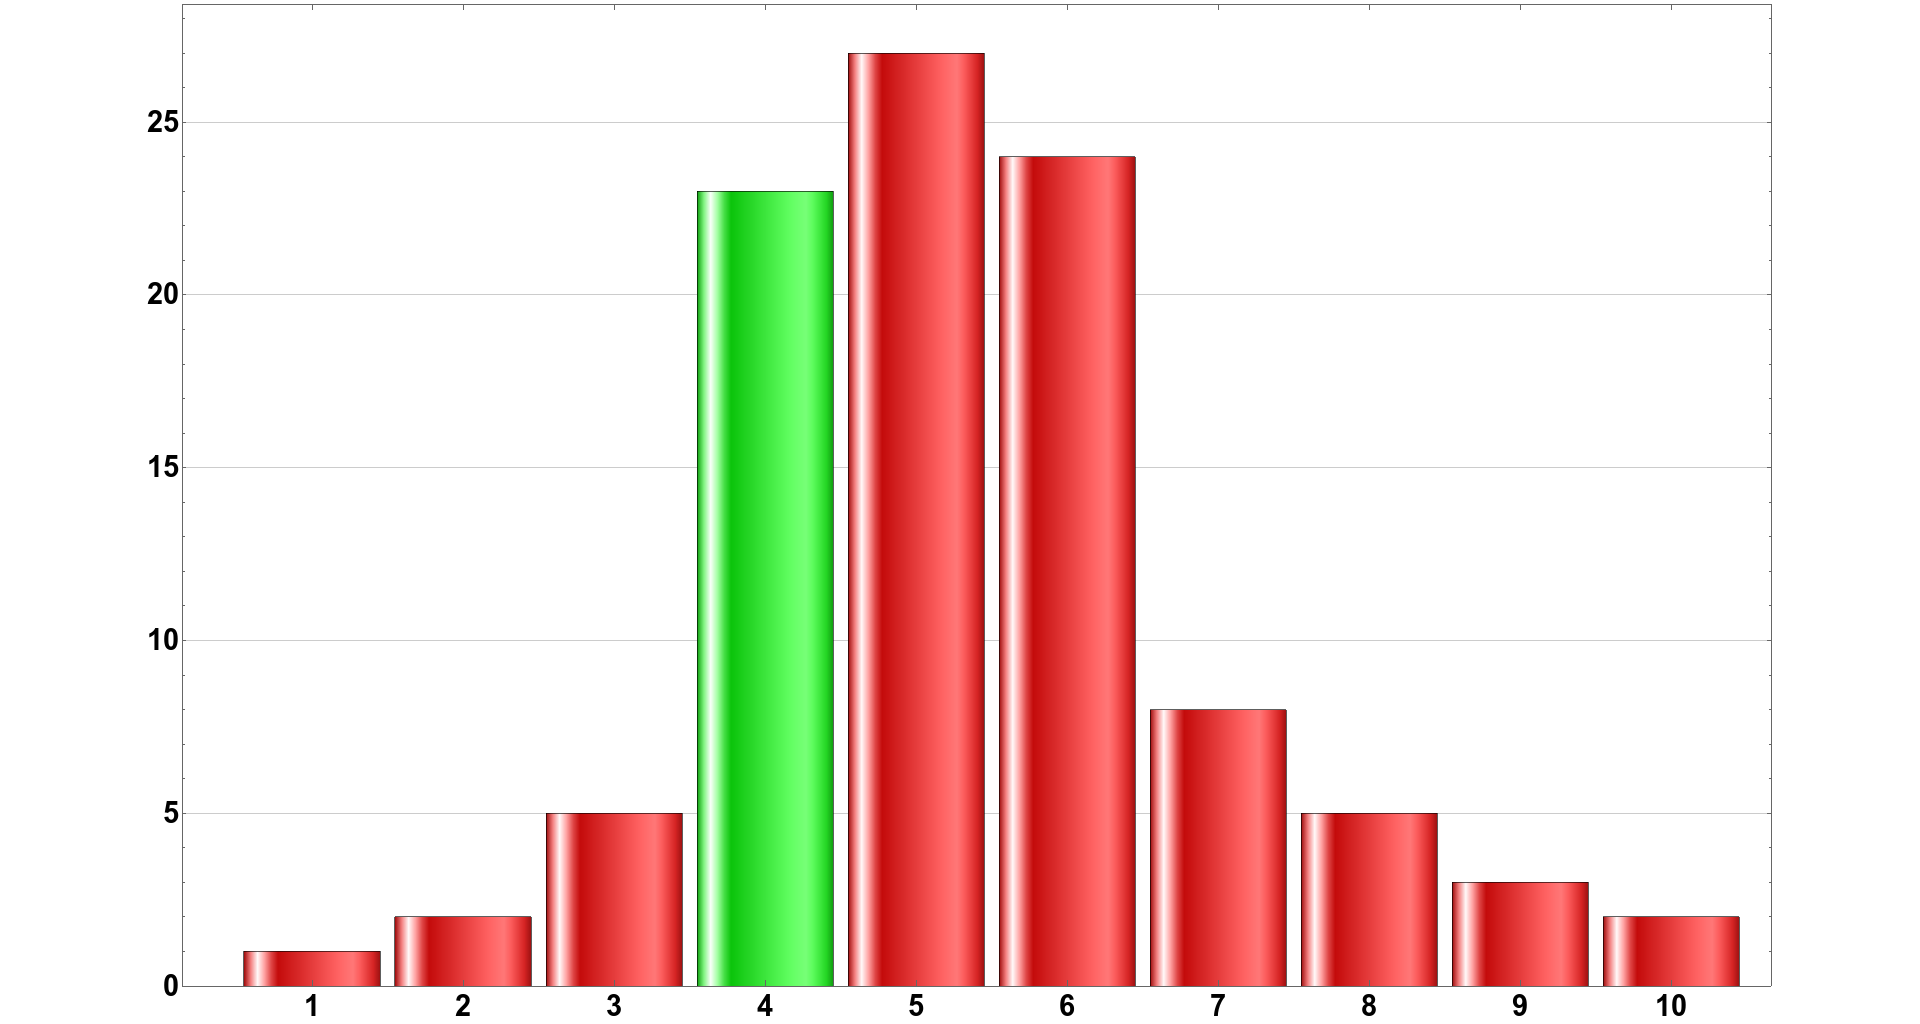
\includegraphics[width=\columnwidth]{images/electric-types.png}\caption{Distribution of Electric Types (\%), Urantia type (4) is marked with green.}\end{figure}}
\vs p049 2:24 \ublistelem{6.}\bibnobreakspace \bibemph{The energizing types.} Not all worlds are alike in the manner of taking in energy. Not all inhabited worlds have an atmospheric ocean suited to respiratory exchange of gases, such as is present on Urantia. During the earlier and the later stages of many planets, beings of your present order could not exist; and when the respiratory factors of a planet are very high or very low, but when all other prerequisites to intelligent life are adequate, the Life Carriers often establish on such worlds a modified form of mortal existence, beings who are competent to effect their life\hyp{}process exchanges directly by means of light\hyp{}energy and the firsthand power transmutations of the Master Physical Controllers.
\vs p049 2:25 There are six differing types of animal and mortal nutrition: The subbreathers employ the first type of nutrition, the marine dwellers the second, the mid\hyp{}breathers the third, as on Urantia. The superbreathers employ the fourth type of energy intake, while the nonbreathers utilize the fifth order of nutrition and energy. The sixth technique of energizing is limited to the midway creatures.
\vs p049 2:26 \ublistelem{7.}\bibnobreakspace \bibemph{The unnamed types.} There are numerous additional physical variations in planetary life, but all of these differences are wholly matters of anatomical modification, physiologic differentiation, and electrochemical adjustment. Such distinctions do not concern the intellectual or the spiritual life.
\usection{Worlds of the Nonbreathers}
\vs p049 3:1 The majority of inhabited planets are peopled with the breathing type of intelligent beings. But there are also orders of mortals who are able to live on worlds with little or no air. Of the Orvonton inhabited worlds this type amounts to less than 7\%. In Nebadon this percentage is less than 3. In all Satania there are only 9 such worlds.
\vs p049 3:2 There are so very few of the nonbreather type of inhabited worlds in Satania because this more recently organized section of Norlatiadek still abounds in meteoric space bodies; and worlds without a protective friction atmosphere are subject to incessant bombardment by these wanderers. Even some of the comets consist of meteor swarms, but as a rule they are disrupted smaller bodies of matter.
\vs p049 3:3 Millions upon millions of meteorites enter the atmosphere of Urantia daily, coming in at the rate of almost 320 km/s. On the nonbreathing worlds the advanced races must do much to protect themselves from meteor damage by making electrical installations which operate to consume or shunt the meteors. Great danger confronts them when they venture beyond these protected zones. These worlds are also subject to disastrous electrical storms of a nature unknown on Urantia. During such times of tremendous energy fluctuation the inhabitants must take refuge in their special structures of protective insulation.
\vs p049 3:4 Life on the worlds of the nonbreathers is radically different from what it is on Urantia. The nonbreathers do not eat food or drink water as do the Urantia races. The reactions of the nervous system, the heat\hyp{}regulating mechanism, and the metabolism of these specialized peoples are radically different from such functions of Urantia mortals. Almost every act of living, aside from reproduction, differs, and even the methods of procreation are somewhat different.
\vs p049 3:5 On the nonbreathing worlds the animal species are radically unlike those found on the atmospheric planets. The nonbreathing plan of life varies from the technique of existence on an atmospheric world; even in survival their peoples differ, being candidates for Spirit fusion. Nevertheless, these beings enjoy life and carry forward the activities of the realm with the same relative trials and joys that are experienced by the mortals living on atmospheric worlds. In mind and character the nonbreathers do not differ from other mortal types.
\vs p049 3:6 You would be more than interested in the planetary conduct of this type of mortal because such a race of beings inhabits a sphere in close proximity to Urantia.
\usection{Evolutionary Will Creatures}
\vs p049 4:1 There are great differences between the mortals of the different worlds, even among those belonging to the same intellectual and physical types, but all mortals of will dignity are erect animals, bipeds.
\vs p049 4:2 There are six basic evolutionary races: three primary --- red, yellow, and blue; and three secondary --- orange, green, and indigo. Most inhabited worlds have all of these races, but many of the three\hyp{}brained planets harbour only the three primary types. Some local systems also have only these three races.
\vs p049 4:3 The average special physical\hyp{}sense endowment of human beings is 12\fnst{\textbf{12}, It was Rudolf Steiner who first suggested the idea of 12 senses. His theory was later developed by others, e.g. Appli, Kranich, Schoorel, Soesman et al. Steiner's 12 senses are grouped as follows:\begin{itemize}\item Lower (0-7 years): life, touch, movement, balance. \item Feeling (7-14 years): sight, smell, taste, warmth. \item Cognitive (14-21 years): hearing, speech, thought, ego.\end{itemize} On the other hand, these are not all \bibemph{physical} senses, which are probably more accurately mapped to the 12 \bibemph{cranial nerves}: olfactory, optic, motor oculi, patheticus, tri\hyp{}facial, abducens, facial nerve, auditory, glossopharyngeal, pneumogastric, spinal accessory, hypoglossal. But the number of cranial nerves is always exact, so why does the text refer to the \bibemph{average} endowment?}, though the special senses of the three\hyp{}brained mortals are extended slightly beyond those of the one\hyp{} and two\hyp{}brained types; they can see and hear considerably more than the Urantia races.
\vs p049 4:4 Young are usually born singly, multiple births being the exception, and the family life is fairly uniform on all types of planets. Sex equality prevails on all advanced worlds; male and female are equal in mind endowment and spiritual status. We do not regard a planet as having emerged from barbarism so long as one sex seeks to tyrannize over the other. This feature of creature experience is always greatly improved after the arrival of a Material Son and Daughter.
\vs p049 4:5 \pc Seasons and temperature variations occur on all sunlighted and sun\hyp{}heated planets. Agriculture is universal on all atmospheric worlds; tilling the soil is the one pursuit that is common to the advancing races of all such planets.
\vs p049 4:6 Mortals all have the same general struggles with microscopic foes in their early days, such as you now experience on Urantia, though perhaps not so extensive. The length of life varies on the different planets from 25 years on the primitive worlds to near 500 on the more advanced and older spheres.
\vs p049 4:7 Human beings are all gregarious, both tribal and racial. These group segregations are inherent in their origin and constitution. Such tendencies can be modified only by advancing civilization and by gradual spiritualization. The social, economic, and governmental problems of the inhabited worlds vary in accordance with the age of the planets and the degree to which they have been influenced by the successive sojourns of the divine Sons.
\vs p049 4:8 \pc Mind is the bestowal of the Infinite Spirit and functions quite the same in diverse environments. The mind of mortals is akin, regardless of certain structural and chemical differences which characterize the physical natures of the will creatures of the local systems. Regardless of personal or physical planetary differences, the mental life of all these various orders of mortals is very similar, and their immediate careers after death are very much alike.
\vs p049 4:9 But mortal mind without immortal spirit cannot survive. The mind of man is mortal; only the bestowed spirit is immortal. Survival is dependent on spiritualization by the ministry of the Adjuster --- on the birth and evolution of the immortal soul; at least, there must not have developed an antagonism towards the Adjuster’s mission of effecting the spiritual transformation of the material mind.
\usection{The Planetary Series of Mortals}
\vs p049 5:1 It will be somewhat difficult to make an adequate portrayal of the planetary series of mortals because you know so little about them, and because there are so many variations. Mortal creatures may, however, be studied from numerous viewpoints, among which are the following:
\vs p049 5:2 \ublistelem{1.}\bibnobreakspace Adjustment to planetary environment.
\vs p049 5:3 \ublistelem{2.}\bibnobreakspace Brain\hyp{}type series.
\vs p049 5:4 \ublistelem{3.}\bibnobreakspace Spirit\hyp{}reception series.
\vs p049 5:5 \ublistelem{4.}\bibnobreakspace Planetary\hyp{}mortal epochs.
\vs p049 5:6 \ublistelem{5.}\bibnobreakspace Creature\hyp{}kinship serials.
\vs p049 5:7 \ublistelem{6.}\bibnobreakspace Adjuster\hyp{}fusion series.
\vs p049 5:8 \ublistelem{7.}\bibnobreakspace Techniques of terrestrial escape.
\vs p049 5:9 \pc The inhabited spheres of the seven superuniverses are peopled with mortals who simultaneously classify in some one or more categories of each of these seven generalized classes of evolutionary creature life. But even these general classifications make no provision for such beings as midsoniters nor for certain other forms of intelligent life. The inhabited worlds, as they have been presented in these narratives, are peopled with evolutionary mortal creatures, but there are other life forms.
\vs p049 5:10 \ublistelem{1.}\bibnobreakspace \bibemph{Adjustment to planetary environment.} There are three general groups of inhabited worlds from the standpoint of the adjustment of creature life to the planetary environment: the normal adjustment group, the radical adjustment group, and the experimental group.
\vs p049 5:11 Normal adjustments to planetary conditions follow the general physical patterns previously considered. The worlds of the nonbreathers typify the radical or extreme adjustment, but other types are also included in this group. Experimental worlds are usually ideally adapted to the typical life forms, and on these decimal planets the Life Carriers attempt to produce beneficial variations in the standard life designs. Since your world is an experimental planet, it differs markedly from its sister spheres in Satania; many forms of life have appeared on Urantia that are not found elsewhere; likewise are many common species absent from your planet.
\vs p049 5:12 In the universe of Nebadon, all the life\hyp{}modification worlds are serially linked together and constitute a special domain of universe affairs which is given attention by designated administrators; and all of these experimental worlds are periodically inspected by a corps of universe directors whose chief is the veteran finaliter known in Satania as Tabamantia.
\vs p049 5:13 \ublistelem{2.}\bibnobreakspace \bibemph{Brain\hyp{}type series.} The one physical uniformity of mortals is the brain and nervous system; nevertheless, there are three basic organizations of the brain mechanism: the one-, the two-, and the three\hyp{}brained types. Urantians are of the two\hyp{}brained type\fnst{\textbf{Urantians are of the two\hyp{}brained type}, The two conjectures on the identification of these ``two brains'' were: a) the two hemispheres of the cerebral cortex and b) the brain proper and the spinal cord. Both conjectures turned out to be wrong after careful examination of Dr William~S. Sadler's ``Physiology of Faith and Fear'', Chicago, 1912 (pp.~513--514), where the first brain is identified with the brain proper (including medulla oblongata and the spinal cord) and the second brain is the \emph{solar plexus}, also referred to as \emph{the ``abdominal brain''}.}, somewhat more imaginative, adventurous, and philosophical than the one\hyp{}brained mortals but somewhat less spiritual, ethical, and worshipful than the three\hyp{}brained orders. These brain differences characterize even the prehuman animal existences.
\vs p049 5:14 From the two\hyp{}hemisphere type of the Urantian cerebral cortex you can, by analogy, grasp something of the one\hyp{}brained type. The third brain of the three\hyp{}brained orders is best conceived as an evolvement of your lower or rudimentary form of brain, which is developed to the point where it functions chiefly in control of physical activities, leaving the two superior brains free for higher engagements: one for intellectual functions and the other for the spiritual\hyp{}counterparting activities of the Thought Adjuster.
\vs p049 5:15 While the terrestrial attainments of the one\hyp{}brained races are slightly limited in comparison with the two\hyp{}brained orders, the older planets of the three\hyp{}brained group exhibit civilizations that would astound Urantians, and which would somewhat shame yours by comparison. In mechanical development and material civilization, even in intellectual progress, the two\hyp{}brained mortal worlds are able to equal the three\hyp{}brained spheres. But in the higher control of mind and development of intellectual and spiritual reciprocation, you are somewhat inferior.
\vs p049 5:16 All such comparative estimates concerning the intellectual progress or the spiritual attainments of any world or group of worlds should in fairness recognize planetary age; much, very much, depends on age, the help of the biologic uplifters, and the subsequent missions of the various orders of the divine Sons.
\vs p049 5:17 While the three\hyp{}brained peoples are capable of a slightly higher planetary evolution than either the one\hyp{} or two\hyp{}brained orders, all have the same type of life plasm and carry on planetary activities in very similar ways, much as do human beings on Urantia. These three types of mortals are distributed throughout the worlds of the local systems. In the majority of cases planetary conditions had very little to do with the decisions of the Life Carriers to project these varied orders of mortals on the different worlds; it is a prerogative of the Life Carriers thus to plan and execute.
\vs p049 5:18 These three orders stand on an equal footing in the ascension career. Each must traverse the same intellectual scale of development, and each must master the same spiritual tests of progression. The system administration and the constellation overcontrol of these different worlds are uniformly free from discrimination; even the regimes of the Planetary Princes are identical.
\vs p049 5:19 \ublistelem{3.}\bibnobreakspace \bibemph{Spirit\hyp{}reception series.} There are three groups of mind design as related to contact with spirit affairs. This classification does not refer to the one-, two-, and three\hyp{}brained orders of mortals; it refers primarily to gland chemistry, more particularly to the organization of certain glands comparable to the pituitary bodies. The races on some worlds have one gland, on others two, as do Urantians\fnst{\textbf{two, as do Urantians}, my original conjecture was that the second gland here referred to is in fact the pineal gland or epiphysis. The hypophysis and epiphysis correspond to the 6\ts{th} and 7\ts{th} chakras, which in the Urantia Papers are called ``adjutant mind\hyp{}spirits'', so the ``opening of the 3\ts{rd} eye'' (enlightenment) would correspond to the synchronized action of the two higher adjutants (worship and wisdom), coordinating the lower chakra activities. However, in his book ``The Truth About Spiritualism'' (1923, pp.40--41), Dr~William Sadler mentions the anterior and posterior lobes of the human pituitary gland. He also notes: \bibemph{``man possesses a larger anterior lobe and is therefore more gifted in analytical reason and more reliable in mature judgment; but woman, because of this fact that she has a superior posterior lobe of the pituitary gland, has more ability when it comes to sizing up and prognosticating human character.''}}, while on still other spheres the races have three of these unique bodies. The inherent imagination and spiritual receptivity is definitely influenced by this differential chemical endowment.
\vs p049 5:20 Of the spirit\hyp{}reception types, 65\% are of the second group, like the Urantia races. 12\% are of the first type, naturally less receptive, while 23\% are more spiritually inclined during terrestrial life. But such distinctions do not survive natural death; all of these racial differences pertain only to the life in the flesh.\tunemarkup{pictures}{\begin{figure}[H]\centering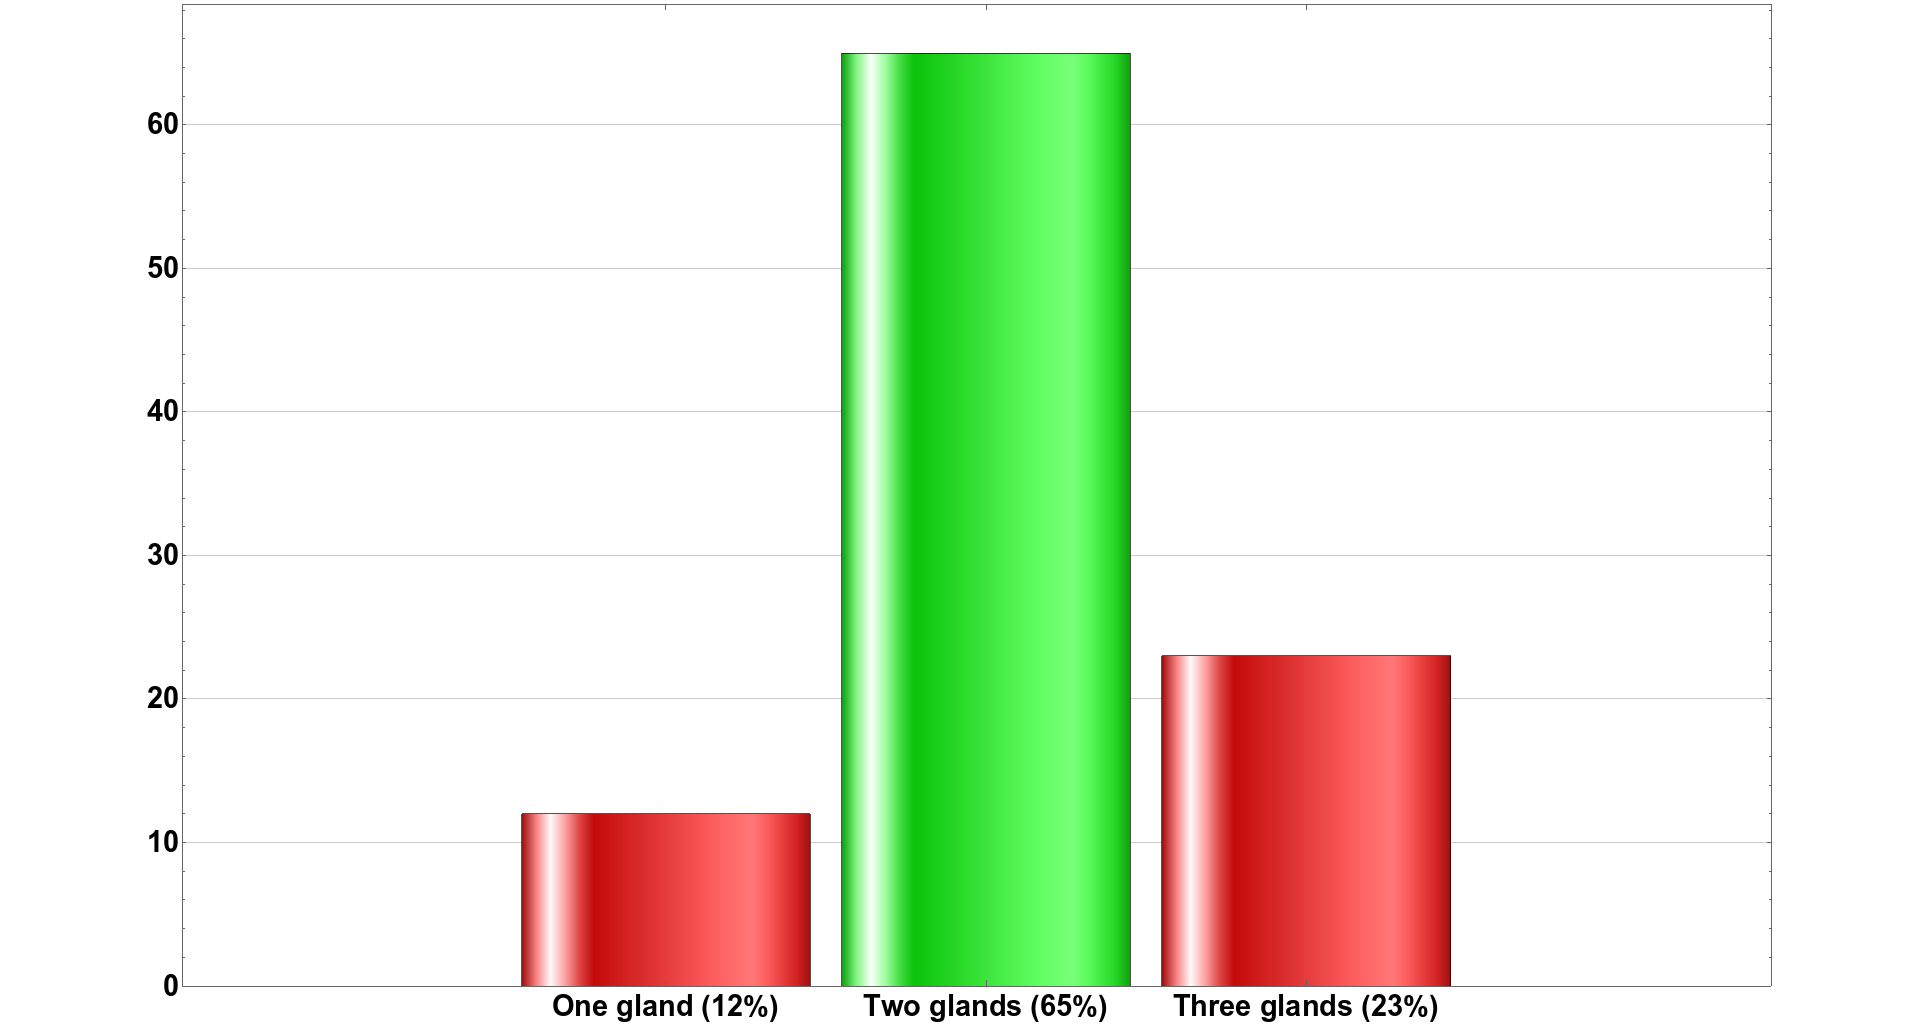
\includegraphics[width=\columnwidth]{images/spirit-reception-types.png}\caption{Distribution of Spirit Reception Types (\%), Urantia type (``Two glands'') is marked with green.}\end{figure}}
\vs p049 5:21 \ublistelem{4.}\bibnobreakspace \bibemph{Planetary\hyp{}mortal epochs.} This classification recognizes the succession of temporal dispensations as they affect man’s terrestrial status and his reception of celestial ministry.
\vs p049 5:22 Life is initiated on the planets by the Life Carriers, who watch over its development until sometime after the evolutionary appearance of mortal man. Before the Life Carriers leave a planet, they duly install a Planetary Prince as ruler of the realm. With this ruler there arrives a full quota of subordinate auxiliaries and ministering helpers, and the first adjudication of the living and the dead is simultaneous with his arrival.
\vs p049 5:23 With the emergence of human groupings, this Planetary Prince arrives to inaugurate human civilization and to focalize human society. Your world of confusion is no criterion of the early days of the reign of the Planetary Princes, for it was near the beginning of such an administration on Urantia that your Planetary Prince, Caligastia, cast his lot with the rebellion of the System Sovereign, Lucifer. Your planet has pursued a stormy course ever since.
\vs p049 5:24 On a normal evolutionary world, racial progress attains its natural biologic peak during the regime of the Planetary Prince, and shortly thereafter the System Sovereign dispatches a Material Son and Daughter to that planet. These imported beings are of service as biologic uplifters; their default on Urantia further complicated your planetary history.
\vs p049 5:25 When the intellectual and ethical progress of a human race has reached the limits of evolutionary development, there comes an Avonal Son of Paradise on a magisterial mission; and later on, when the spiritual status of such a world is nearing its limit of natural attainment, the planet is visited by a Paradise bestowal Son. The chief mission of a bestowal Son is to establish the planetary status, release the Spirit of Truth for planetary function, and thus effect the universal coming of the Thought Adjusters.
\vs p049 5:26 Here, again, Urantia deviates: There has never been a magisterial mission on your world, neither was your bestowal Son of the Avonal order; your planet enjoyed the signal honour of becoming the mortal home planet of the Sovereign Son, Michael of Nebadon.
\vs p049 5:27 As a result of the ministry of all the successive orders of divine sonship, the inhabited worlds and their advancing races begin to approach the apex of planetary evolution. Such worlds now become ripe for the culminating mission, the arrival of the Trinity Teacher Sons. This epoch of the Teacher Sons is the vestibule to the final planetary age --- evolutionary utopia --- the age of light and life.
\vs p049 5:28 This classification of human beings will receive particular attention in a succeeding paper.
\vs p049 5:29 \ublistelem{5.}\bibnobreakspace \bibemph{Creature\hyp{}kinship serials.} Planets are not only organized vertically into systems, constellations, and so on, but the universe administration also provides for horizontal groupings according to type, series, and other relationships. This lateral administration of the universe pertains more particularly to the co\hyp{}ordination of activities of a kindred nature which have been independently fostered on different spheres. These related classes of universe creatures are periodically inspected by certain composite corps of high personalities presided over by long\hyp{}experienced finaliters.
\vs p049 5:30 These kinship factors are manifest on all levels, for kinship serials exist among nonhuman personalities as well as among mortal creatures --- even between human and superhuman orders. Intelligent beings are vertically related in 12 great groups of 7 major divisions each. The co\hyp{}ordination of these uniquely related groups of living beings is probably effected by some not fully comprehended technique of the Supreme Being.
\vs p049 5:31 \ublistelem{6.}\bibnobreakspace \bibemph{Adjuster\hyp{}fusion series.} The spiritual classification or grouping of all mortals during their prefusion experience is wholly determined by the relation of the personality status to the indwelling Mystery Monitor. Almost 90\% of the inhabited worlds of Nebadon are peopled with Adjuster\hyp{}fusion mortals in contrast with a near\hyp{}by universe where scarcely more than one half of the worlds harbour beings who are Adjuster\hyp{}indwelt candidates for eternal fusion.
\vs p049 5:32 \ublistelem{7.}\bibnobreakspace \bibemph{Techniques of terrestrial escape.} There is fundamentally only one way in which individual human life can be initiated on the inhabited worlds, and that is through creature procreation and natural birth; but there are numerous techniques whereby man escapes his terrestrial status and gains access to the inward moving stream of Paradise ascenders.
\usection{Terrestrial Escape}
\vs p049 6:1 All of the differing physical types and planetary series of mortals alike enjoy the ministry of Thought Adjusters, guardian angels, and the various orders of the messenger hosts of the Infinite Spirit. All alike are liberated from the bonds of flesh by the emancipation of natural death, and all alike go thence to the morontia worlds of spiritual evolution and mind progress.
\vs p049 6:2 From time to time, on motion of the planetary authorities or the system rulers, special resurrections of the sleeping survivors are conducted. Such resurrections occur at least every millennium of planetary time, when not all but “many of those who sleep in the dust awake.” These special resurrections are the occasion for mobilizing special groups of ascenders for specific service in the local universe plan of mortal ascension. There are both practical reasons and sentimental associations connected with these special resurrections.
\vs p049 6:3 Throughout the earlier ages of an inhabited world, many are called to the mansion spheres at the special and the millennial resurrections, but most survivors are repersonalized at the inauguration of a new dispensation associated with the advent of a divine Son of planetary service.
\vs p049 6:4 \ublistelem{1.}\bibnobreakspace \bibemph{Mortals of the dispensational or group order of survival.} With the arrival of the first Adjuster on an inhabited world the guardian seraphim also make their appearance; they are indispensable to terrestrial escape. Throughout the life\hyp{}lapse period of the sleeping survivors the spiritual values and eternal realities of their newly evolved and immortal souls are held as a sacred trust by the personal or by the group guardian seraphim.
\vs p049 6:5 The group guardians of assignment to the sleeping survivors always function with the judgment Sons on their world advents. “He shall send his angels, and they shall gather together his elect from the four winds.” With each seraphim of assignment to the repersonalization of a sleeping mortal there functions the returned Adjuster, the same immortal Father fragment that lived in him during the days in the flesh, and thus is identity restored and personality resurrected. During the sleep of their subjects these waiting Adjusters serve on Divinington; they never indwell another mortal mind in this interim.
\vs p049 6:6 While the older worlds of mortal existence harbour those highly developed and exquisitely spiritual types of human beings who are virtually exempt from the morontia life, the earlier ages of the animal\hyp{}origin races are characterized by primitive mortals who are so immature that fusion with their Adjusters is impossible. The reawakening of these mortals is accomplished by the guardian seraphim in conjunction with an individualized portion of the immortal spirit of the Third Source and Centre.
\vs p049 6:7 Thus are the sleeping survivors of a planetary age repersonalized in the dispensational roll calls. But with regard to the nonsalvable personalities of a realm, no immortal spirit is present to function with the group guardians of destiny, and this constitutes cessation of creature existence. While some of your records have pictured these events as taking place on the planets of mortal death, they all really occur on the mansion worlds.
\vs p049 6:8 \ublistelem{2.}\bibnobreakspace \bibemph{Mortals of the individual orders of ascension.} The individual progress of human beings is measured by their successive attainment and traversal (mastery) of the seven cosmic circles. These circles of mortal progression are levels of associated intellectual, social, spiritual, and cosmic\hyp{}insight values. Starting out in the seventh circle, mortals strive for the first, and all who have attained the third immediately have personal guardians of destiny assigned to them. These mortals may be repersonalized in the morontia life independent of dispensational or other adjudications.
\vs p049 6:9 Throughout the earlier ages of an evolutionary world, few mortals go to judgment on the third day. But as the ages pass, more and more the personal guardians of destiny are assigned to the advancing mortals, and thus increasing numbers of these evolving creatures are repersonalized on the first mansion world on the third day after natural death. On such occasions the return of the Adjuster signalizes the awakening of the human soul, and this is the repersonalization of the dead just as literally as when the en masse roll is called at the end of a dispensation on the evolutionary worlds.
\vs p049 6:10 There are three groups of individual ascenders: The less advanced land on the initial or first mansion world. The more advanced group may take up the morontia career on any of the intermediate mansion worlds in accordance with previous planetary progression. The most advanced of these orders really begin their morontia experience on the seventh mansion world.
\vs p049 6:11 \ublistelem{3.}\bibnobreakspace \bibemph{Mortals of the probationary\hyp{}dependent orders of ascension.} The arrival of an Adjuster constitutes identity in the eyes of the universe, and all indwelt beings are on the roll calls of justice. But temporal life on the evolutionary worlds is uncertain, and many die in youth before choosing the Paradise career. Such Adjuster\hyp{}indwelt children and youths follow the parent of most advanced spiritual status, thus going to the system finaliter world (the probationary nursery) on the third day, at a special resurrection, or at the regular millennial and dispensational roll calls.
\vs p049 6:12 Children who die when too young to have Thought Adjusters are repersonalized on the finaliter world of the local systems concomitant with the arrival of either parent on the mansion worlds. A child acquires physical entity at mortal birth, but in the matter of survival all Adjusterless children are reckoned as still attached to their parents.
\vs p049 6:13 In due course Thought Adjusters come to indwell these little ones, while the seraphic ministry to both groups of the probationary\hyp{}dependent orders of survival is in general similar to that of the more advanced parent or is equivalent to that of the parent in case only one survives. Those attaining the third circle, regardless of the status of their parents, are accorded personal guardians.
\vs p049 6:14 Similar probation nurseries are maintained on the finaliter spheres of the constellation and the universe headquarters for the Adjusterless children of the primary and secondary modified orders of ascenders.
\vs p049 6:15 \ublistelem{4.}\bibnobreakspace \bibemph{Mortals of the secondary modified orders of ascension.} These are the progressive human beings of the intermediate evolutionary worlds. As a rule they are not immune to natural death, but they are exempt from passing through the seven mansion worlds.
\vs p049 6:16 The less perfected group reawaken on the headquarters of their local system, passing by only the mansion worlds. The intermediate group go to the constellation training worlds; they pass by the entire morontia regime of the local system. Still farther on in the planetary ages of spiritual striving, many survivors awaken on the constellation headquarters and there begin the Paradise ascent.
\vs p049 6:17 But before any of these groups may go forward, they must journey back as instructors to the worlds they missed, gaining many experiences as teachers in those realms which they passed by as students. They all subsequently proceed to Paradise by the ordained routes of mortal progression.
\vs p049 6:18 \ublistelem{5.}\bibnobreakspace \bibemph{Mortals of the primary modified order of ascension.} These mortals belong to the Adjuster\hyp{}fused type of evolutionary life, but they are most often representative of the final phases of human development on an evolving world. These glorified beings are exempt from passing through the portals of death; they are submitted to Son seizure; they are translated from among the living and appear immediately in the presence of the Sovereign Son on the headquarters of the local universe.
\vs p049 6:19 These are the mortals who fuse with their Adjusters during mortal life, and such Adjuster\hyp{}fused personalities traverse space freely before being clothed with morontia forms. These fused souls go by direct Adjuster transit to the resurrection halls of the higher morontia spheres, where they receive their initial morontia investiture just as do all other mortals arriving from the evolutionary worlds.
\vs p049 6:20 This primary modified order of mortal ascension may apply to individuals in any of the planetary series from the lowest to the highest stages of the Adjuster\hyp{}fusion worlds, but it more frequently functions on the older of these spheres after they have received the benefits of numerous sojourns of the divine Sons.
\vs p049 6:21 With the establishment of the planetary era of light and life, many go to the universe morontia worlds by the primary modified order of translation. Further along in the advanced stages of settled existence, when the majority of the mortals leaving a realm are embraced in this class, the planet is regarded as belonging to this series. Natural death becomes decreasingly frequent on these spheres long settled in light and life.
\vsetoff
\vs p049 6:22 [Presented by a Melchizedek of the Jerusem School of Planetary Administration.]
\quizlink
